\documentclass[border=10pt,12pt]{standalone}

\usepackage{pgf}
\usepackage{tikz}
\usetikzlibrary{arrows,shapes,snakes,automata,backgrounds,petri}

\begin{document}

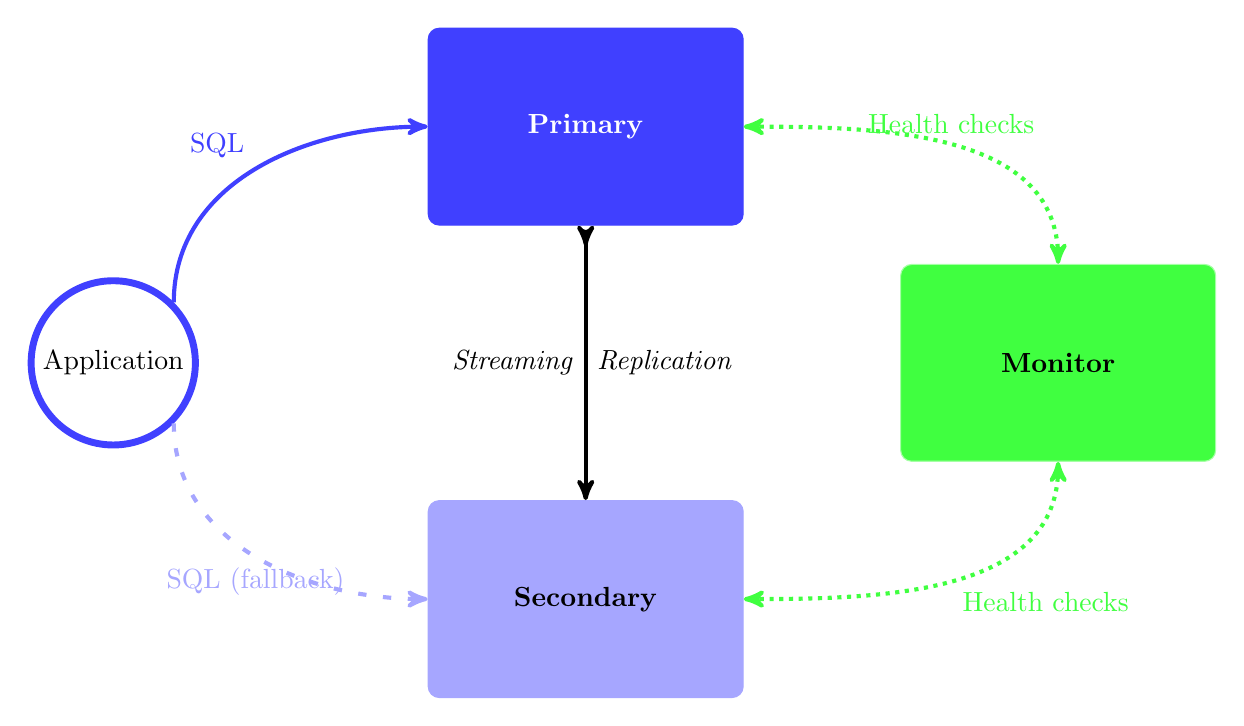
\begin{tikzpicture}[>=stealth',bend angle=45,auto,rounded corners]

  \tikzstyle{app}=[circle,thick,draw=blue!75,fill=white,line width=0.25em]
  \tikzstyle{primary}=[rectangle,color=white,draw=blue!75,fill=blue!75,
    minimum height=2.5cm,minimum width=4cm]
  \tikzstyle{standby}=[draw=blue!35,fill=blue!35,
    minimum height=2.5cm,minimum width=4cm]
  \tikzstyle{monitor}=[draw=green!35,fill=green!75,
    minimum height=2.5cm,minimum width=4cm]

  %% \draw [help lines] (-10,0) grid (10,20);
  
  \node  (p)   at (0,18)   [primary]       {\textbf{Primary}};
  \node  (s)   at (0,12)   [standby]       {\textbf{Secondary}};
  \node  (app) at (-6,15)  [app]           {Application};
  \node  (m)   at (6,15)   [monitor]       {\textbf{Monitor}};

  \tikzstyle{sql}=[->,color=blue!75,line width=0.15em]
  \tikzstyle{sqlf}=[->,color=blue!35,line width=0.15em,loosely dashed]
  \tikzstyle{sr}=[>->,line width=0.15em]
  \tikzstyle{hc}=[<->,color=green!75,line width=0.15em,dotted]

  \path (app.north east) edge [sql,out=90,in=180]   node {SQL} (p)
        (app.south east) edge [sqlf,out=-90,in=180] node[below] {SQL (fallback)} (s)
        (p)   edge [sr]
                                     node[left]   {\textit{Streaming}}
                                     node [right] {\textit{Replication}} (s)
        (m)   edge [hc,out=90,in=0]  node[above] {Health checks}         (p)
              edge [hc,out=-90,in=0] node        {Health checks}         (s);
\end{tikzpicture}

\end{document}
